\mode*
\part{Working With Files}
\lecture{Files}{files}

\section{Files}
\label{sec:file}

\begin{frame}{File}{A logical view of information storage}
  \begin{block}{User's view}
    A file is the smallest storage unit on disk.
    \begin{itemize}
    \item Data cannot be written to disk unless they are within a file
    \end{itemize}
  \end{block}
  \begin{block}{UNIX view}
    Each file is a sequence of 8-bit bytes
    \begin{itemize}
    \item It's up to the application program to interpret this byte stream.
    \end{itemize}
  \end{block}
\end{frame}

\begin{frame}{File}{What is stored in a file?}
  Source code, object files, executable files, shell scripts, PostScript...
  \begin{block}{Different type of files have different structure}
    \begin{itemize}
    \item UNIX looks at contents to determine type
      \begin{description}
      \item[Shell scripts] start with ``\texttt{\#!}''
      \item[PDF] start with ``\texttt{\%PDF...}''
      \item[Executables] start with \alert{magic number}
      \end{description}
    \item Windows uses file naming conventions
      \begin{description}
      \item[executables] end with ``\texttt{.exe}'' and ``\texttt{.com}''
      \item[MS-Word] end with ``\texttt{.doc}''
      \item[MS-Excel] end with ``\texttt{.xls}''
      \end{description}
    \end{itemize}
  \end{block}
\end{frame}

\begin{frame}{File Types}
  \begin{description}
  \item[Regular files:] ASCII, binary
  \item[Directories:] Maintaining the structure of the FS
  \end{description}
  \begin{block}{In UNIX, everything is a file}
    \begin{description}
    \item[Character special files:] I/O related, such as terminals, printers ...
    \item[Block special files:] Devices that can contain file systems, i.e. disks
      \begin{itemize}
      \item[Disks] --- logically, linear collections of blocks; disk driver translates
        them into physical block addresses
      \end{itemize}
    \end{description}
  \end{block}
\end{frame}

\begin{frame}{File Operations}{POSIX file system calls}%[squeeze]
  \begin{tabular}{>{\ttfamily}l|>{\ttfamily}l}
    creat(name, mode)&read(fd, buffer, byte\_count)\\
    open(name, flags)&write(fd, buffer, byte\_count)\\
    close(fd)&lseek(fd, offset, whence)\\
    link(oldname, newname)&chown(name, owner, group\\
    unlink(name)&fchown(fd, owner, group)\\        
    truncate(name, size)&chmod(name, mode\\
    ftruncate(fd, size)&fchmod(fd, mode)\\
    stat(name, buffer)&utimes(name, times)\\
    fstat(fd, buffer)&\\
  \end{tabular}
\end{frame}

\begin{frame}
  \begin{minipage}[t]{.53\linewidth}
    \begin{iblock}{\texttt{write()}}
      \begin{center}
        \mode<beamer>{ \includegraphics[width=\textwidth]{write-c} }%
        \mode<article>{\cfile{../src/write.c}}
      \end{center}
    \end{iblock}
    \ttfamily
    \begin{itemize}
    \item[\$] man 2 write
    \item[\$] man 3 write
    \end{itemize}
  \end{minipage}\qquad
  \begin{minipage}[t]{.37\linewidth}
    \begin{iblock}{\texttt{read()}}
      \begin{center}
        \mode<beamer>{ 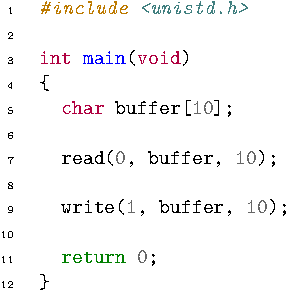
\includegraphics[width=\textwidth]{read-c} }%
        \mode<article>{\cfile{../src/read.c}}
      \end{center}
    \end{iblock}
    \ttfamily
    \begin{itemize}
    \item[\$] man 2 read
    \item[\$] man 3 read
    \end{itemize}
  \end{minipage}
  \vspace*{1em}
  \begin{itemize}
  \item No need to \texttt{open()} \texttt{STDIN}, \texttt{STDOUT}, and \texttt{STDERR}
  \end{itemize}
\end{frame}

\begin{frame}{\cmd{cp}}
  \begin{center}
    \begin{center}
      \mode<beamer>{ 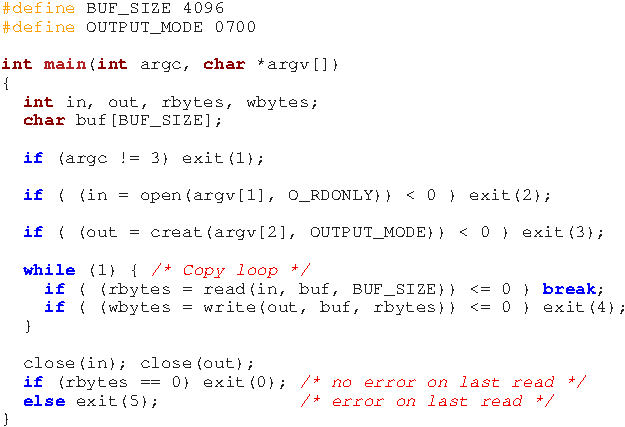
\includegraphics[width=.95\textwidth]{cp-syscall-c} }%
      \mode<article>{\cfile{../src/cp-syscall.c}}
    \end{center}
  \end{center}
\end{frame}

\begin{frame}{\texttt{stdio} --- The Standard I/O Library}
  \begin{description}
  \item[System calls:] \cmd{open(), read(), write(), close()}\ldots
  \item[Library functions:] \cmd{fopen(), fread(), fwrite, fclose()}\ldots
  \end{description}
  \begin{block}{Avoid calling syscalls directly as much as you can}
    \begin{minipage}{.4\linewidth}
      \begin{itemize}
      \item Portability
      \item Buffered I/O
      \end{itemize}
    \end{minipage}\qquad
    \begin{minipage}{.4\linewidth}
      \begin{center}
        \mode<beamer>{ 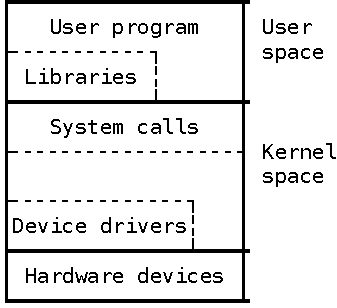
\includegraphics[width=\textwidth]{api} }%
        \mode<article>{ 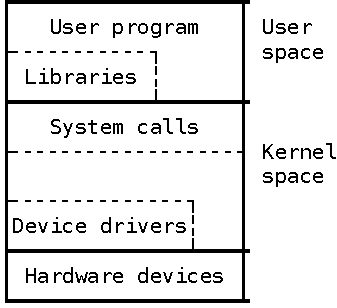
\includegraphics[width=.5\textwidth]{api} }
      \end{center}
    \end{minipage}
  \end{block}  
\end{frame}

\begin{frame}{\texttt{open()} {\scriptsize vs.} \texttt{fopen()}}
  \begin{center}
    \begin{minipage}{.48\linewidth}
      \cmd{open()}\\[1ex]
      \mode<beamer>{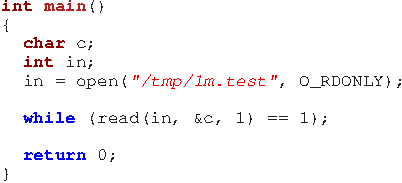
\includegraphics[width=\linewidth]{open-c}\\[1ex]}%
      \mode<article>{\cfile{../src/open.c}}
      \CMD{strace -c ./open}
    \end{minipage}\quad
    \begin{minipage}{.48\linewidth}
      \cmd{fopen()} --- Buffered I/O\\[1ex]
      \mode<beamer>{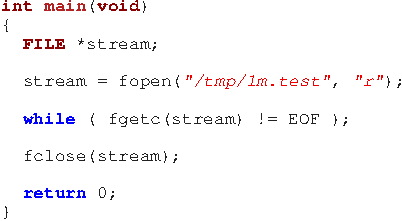
\includegraphics[width=\linewidth]{fopen-c}\\[1ex]}%
      \mode<article>{\cfile{../src/fopen.c}}
      \CMD{strace -c ./fopen}
    \end{minipage}
  \end{center}{\footnotesize
  \begin{itemize}
  \item[\$] \cmd{dd if=/dev/zero of=/tmp/1m.test bs=1k count=1024}
  \end{itemize}}
\end{frame}

\begin{itemize}
\item \url{https://stackoverflow.com/questions/1658476/c-fopen-vs-open}
\end{itemize}

\begin{frame}{\texttt{cp} --- {\small With} \texttt{stdio}}
  \begin{center}
    \mode<beamer>{ 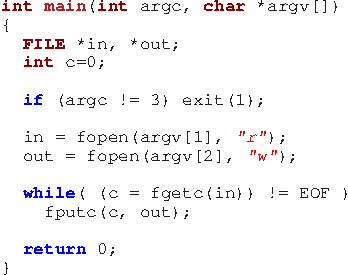
\includegraphics[width=.6\textwidth]{cp-libc-c} }%
    \mode<article>{\cfile{../src/cp-libc.c}}
  \end{center}
  \begin{description}
  \item[\hw] Try \texttt{fread()/fwrite()} instead.
  \end{description}
\end{frame}

\begin{itemize}
\item \url{https://stackoverflow.com/questions/32742430/is-getc-a-macro-or-a-function}
\item \url{https://stackoverflow.com/questions/9104568/macro-vs-function-in-c}
\end{itemize}

\begin{frame}{File System Implementation}
  \begin{iblock}{A typical file system layout}
    \begin{center}
      \mode<beamer>{ \includegraphics[width=\textwidth]{fs-layout} }%
      \mode<article>{ \includegraphics[width=.5\textwidth]{fs-layout} }
    \end{center}
  \end{iblock}
  \begin{center}
    \mode<beamer>{ \includegraphics[width=.8\textwidth]{mbr} }%
    \mode<article>{ \includegraphics[width=.5\textwidth]{mbr} }
  \end{center}
\end{frame}

\begin{frame}{On-Disk Information Structure}
  \begin{description}
  \item[Boot block] a MBR copy
  \item[Superblock] Contains volume details
    \begin{center}
      \begin{tabular}{ll}
        number of blocks& size of blocks\\
        free-block count& free-block pointers\\
        free FCB count& free FCB pointers
      \end{tabular}
    \end{center}
  \item[I-node] Organizes the files \alert{FCB (File Control Block)},
    contains file details (metadata).
  \end{description}
\end{frame}

\begin{frame}
  \begin{block}{Superblock}
    Keeps information about the file system
    \begin{itemize}
    \item Type --- ext2, ext3, ext4...
    \item Size
    \item Status --- how it's mounted, free blocks, free inodes, ...
    \item Information about other metadata structures
    \end{itemize}
  \end{block}
  \begin{itemize}
  \item[\$] \cmd{sudo dumpe2fs /dev/sda1 | less}
  \end{itemize}
\end{frame}

\begin{frame}{Implementing Files}
  \begin{center}
    \mode<beamer>{ 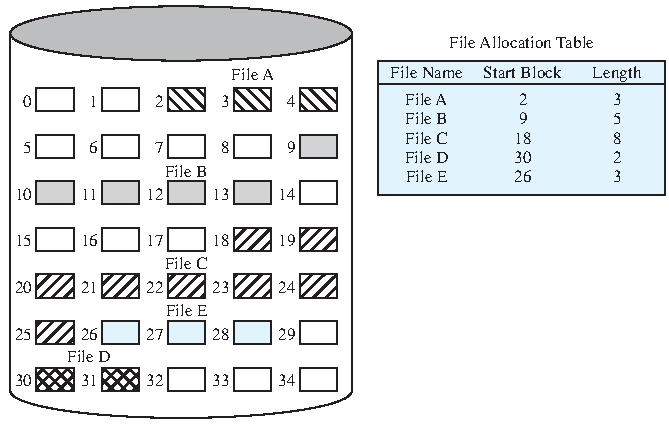
\includegraphics[width=.7\textwidth]{file-alloc-contiguous} }%
    \mode<article>{ 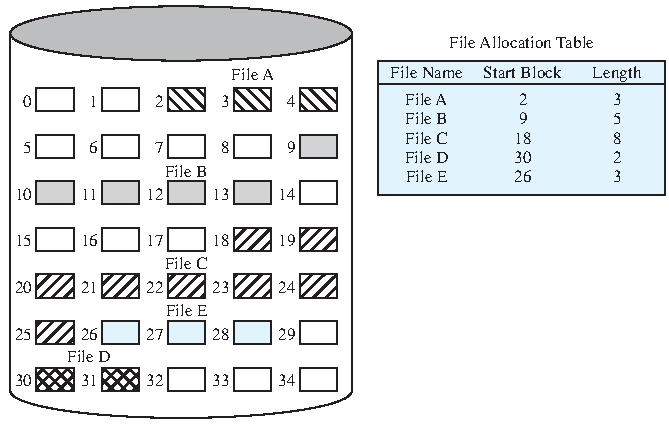
\includegraphics[width=.5\textwidth]{file-alloc-contiguous} }
  \end{center}
  \begin{block}{Contiguous Allocation}
    \begin{multicols}{2}
      \begin{itemize}
      \item[\Good] simple
      \item[\Good] good for read only
      \item[\Bad] fragmentation
      \end{itemize}
    \end{multicols}
  \end{block}
\end{frame}

\begin{frame}
  \begin{center}
    \mode<beamer>{ 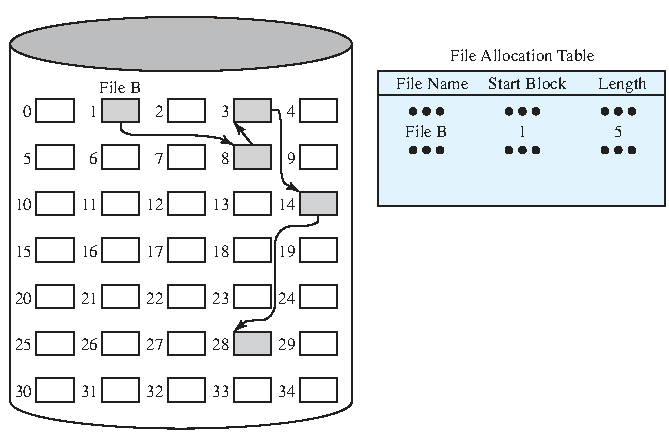
\includegraphics[width=.7\textwidth]{file-alloc-chained} }%
    \mode<article>{ 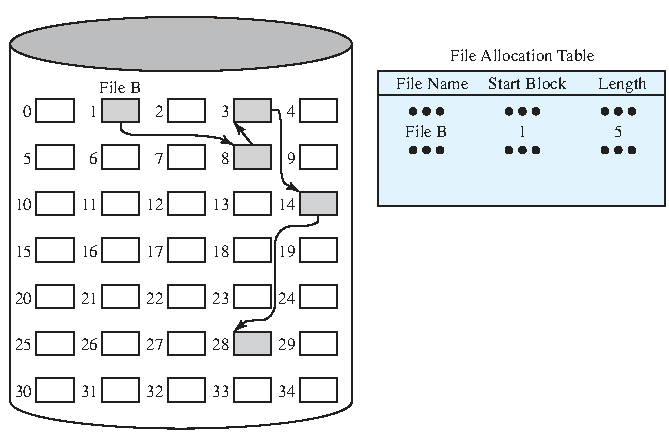
\includegraphics[width=.5\textwidth]{file-alloc-chained} }
  \end{center}
  \begin{block}{Linked List (Chained) Allocation}
    A pointer in each disk block
    \begin{multicols}{2}
      \begin{itemize}
      \item[\Good] no waste block
      \item[\Bad] slow random access
      \item[\Bad] not $2^n$
      \end{itemize}
    \end{multicols}
  \end{block}
\end{frame}

\begin{frame}
  \begin{description}
  \item[Linked List (Chained) Allocation] Though there is no external fragmentation,
    consolidation is still preferred.
  \end{description}
  \begin{center}
    \mode<beamer>{ 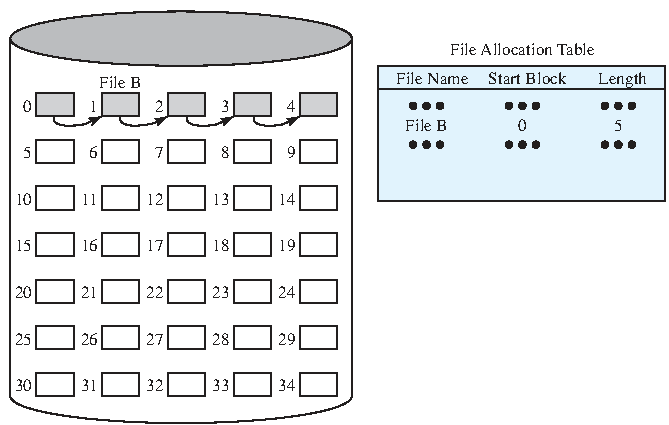
\includegraphics[width=.8\textwidth]{file-alloc-chained2} }%
    \mode<article>{\label{fig:chained2} 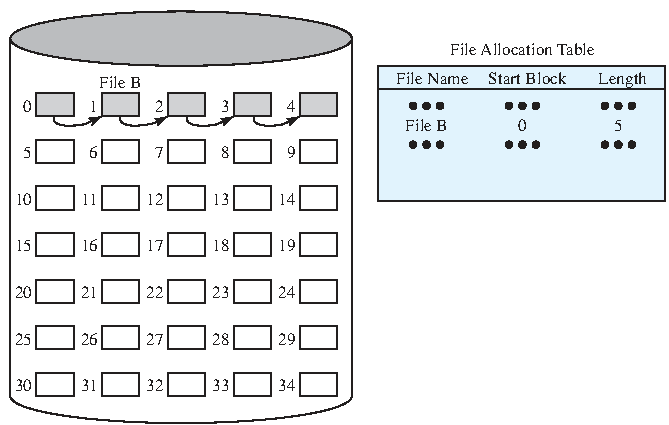
\includegraphics[width=.5\textwidth]{file-alloc-chained2} }
  \end{center}
\end{frame}

\begin{frame}
  \begin{itemize}
  \item[FAT:] Linked list allocation with a table in RAM
  \end{itemize}
  \begin{minipage}{.59\textwidth}
    \begin{block}{}
      \begin{itemize}
      \item Taking the pointer out of each disk block, and putting it into a table in
        memory
      \item fast random access (chain is in RAM)
      \item is $2^n$
      \item the entire table must be in RAM
        $$disk\nearrow{}\Rightarrow FAT\nearrow{}\Rightarrow RAM_{used}\nearrow$$
      \end{itemize}
    \end{block}
  \end{minipage}\quad
  \begin{minipage}{.35\textwidth}
      \mode<beamer>{ \includegraphics[width=\textwidth]{fat} }%
      \mode<article>{ \includegraphics[width=.8\textwidth]{fat} }
  \end{minipage}
\end{frame}

See also: \citetitle[\emph{Wikipedia:FAT}]{wiki:fat}.

\begin{frame}{Indexed Allocation}
  \begin{center}
    \mode<beamer>{ 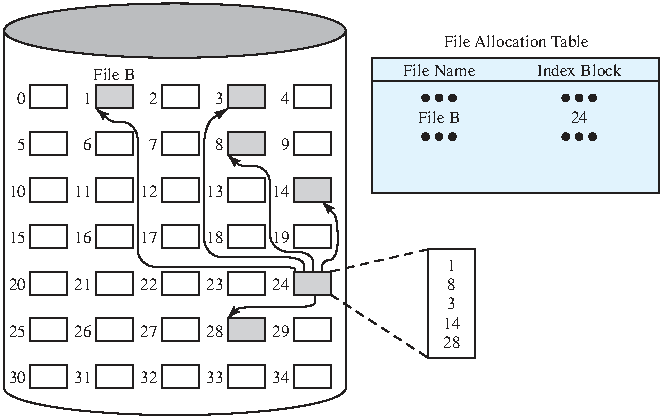
\includegraphics[width=.7\textwidth]{file-alloc-idx} }%
    \mode<article>{ 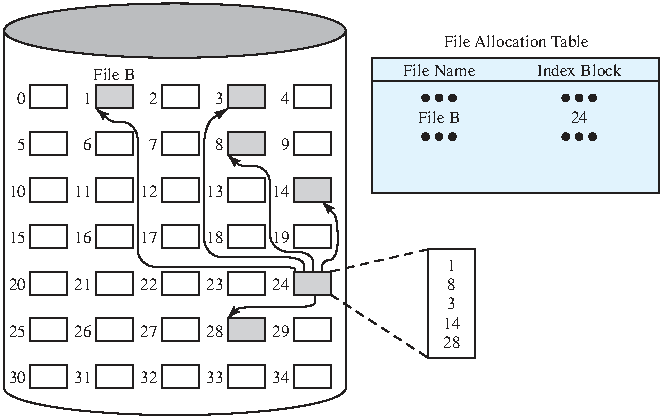
\includegraphics[width=.4\textwidth]{file-alloc-idx} }
  \end{center}
  \begin{description}
  \item[I-node] A data structure for each file. An i-node is in memory \emph{only if} the
    file is open
    $$files_{opened}\nearrow{}\Rightarrow{}RAM_{used}\nearrow{}$$
  \end{description}
\end{frame}

See also: \citetitle[\emph{Wikipedia:inode}]{wiki:inode}.

\begin{frame}<beamer>{I-node}
  \begin{tikzpicture}[remember picture, overlay]
    \node [scale=.8,anchor=south west] at (current page.south west)
    {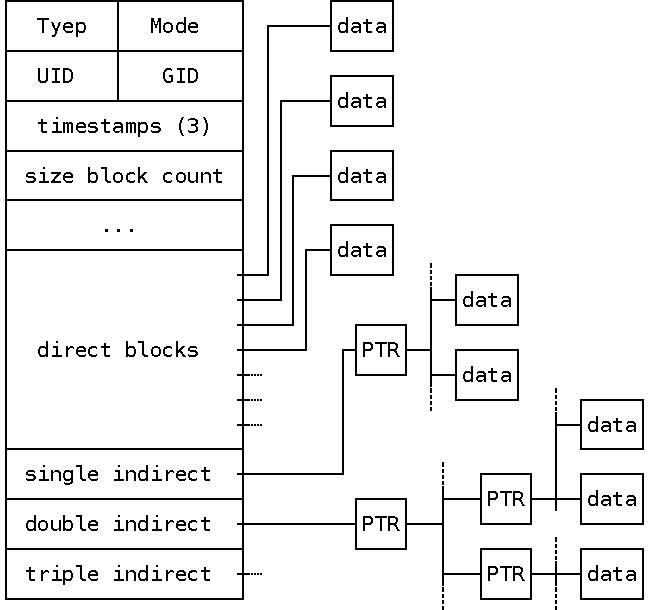
\includegraphics{osc-11-28}};
        
    \node [scale=.7,xshift=-5em,yshift=-5em,anchor=north east,align=left]
    at (current page.north east) {%
      \begin{tabular}{cl}\hline
        \thead{File type}&\thead{Description}\\\hline
        0&Unknown\\
        1&Regular file\\
        2&Directory\\
        3&Character device\\
        4&Block device\\
        5&Named pipe\\
        6&Socket\\
        7&Symbolic link\\\hline
      \end{tabular}\\[1ex]\textbf{Mode:} 9-bit pattern};
  \end{tikzpicture}
\end{frame}

\begin{frame}{UNIX Treats a Directory as a File}
  \mode<article>{\includegraphics[width=.7\textwidth]{inode-struct}}%
  \mode<beamer>{ \hspace{-2.5em}
    \begin{tikzpicture}[remember picture, overlay]
      \node [scale=.29,anchor=south west] at (current page.south west)
      {\includegraphics{inode-struct}};
        
      \node [scale=.7,xshift=-5em,yshift=-5em,anchor=north east] at (current page.north east) {
        \begin{tabular}{|l|l|}
          \hline
          .&2\\\hline
          ..&2\\\hline
          bin&11116545\\\hline
          boot&2\\\hline
          cdrom&12\\\hline
          dev&3\\\hline
          \vdots&\vdots
        \end{tabular}}; 
    \end{tikzpicture}}
\end{frame}

\begin{frame}{\texttt{open()}}
  \begin{description}
    \item[Why?] To avoid constant searching
    \begin{itemize}
    \item Without \texttt{open()}, every file operation involves searching the directory for
      the file.
    \end{itemize}
  \end{description}
  The steps in looking up \texttt{/usr/ast/mbox}
  \begin{center}\label{fig:dir-lookup}
    \mode<beamer>{ 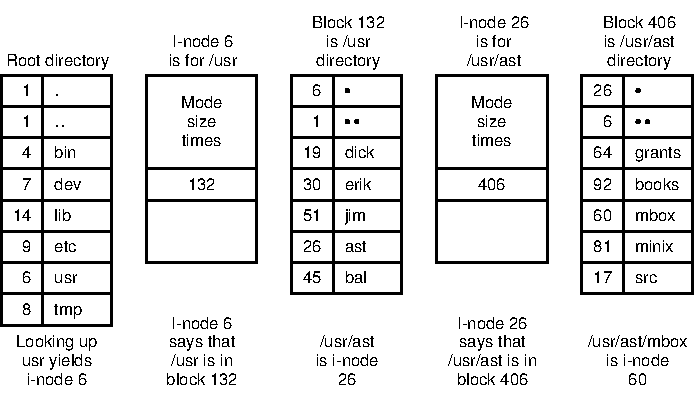
\includegraphics[width=.9\textwidth]{04-35} }%
    \mode<article>{ 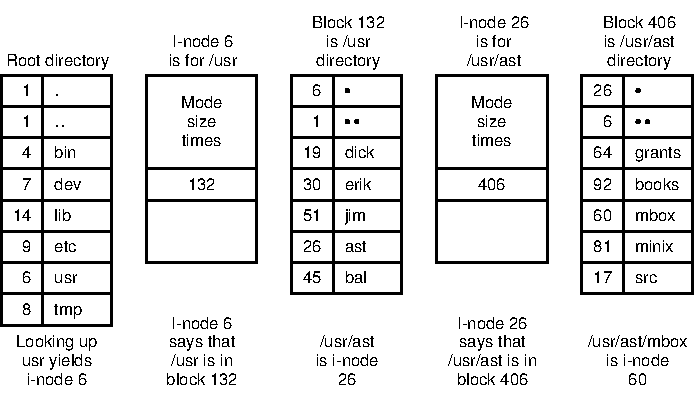
\includegraphics[width=.5\textwidth]{04-35} }
  \end{center}
\end{frame}

\begin{frame}
  \begin{block}{\texttt{fd open(pathname, flags)}}
    \begin{itemize}
    \item[] A per-process \alert{open-file table} is kept in the OS
      \begin{itemize}
      \item upon a successful \texttt{open()} syscall, a new entry is added into this table
      \item indexed by \alert{file descriptor (fd)}
      \item \texttt{close()} to remove an entry from the table
      \end{itemize}
    \item[] To see files opened by a process, e.g. \texttt{init}
      \begin{itemize}
      \item[\$] \cmd{lsof -p 1}
      \end{itemize}
    \end{itemize}
  \end{block}
    \qquad\CMD{man 2 open}
\end{frame}

\begin{frame}
  \begin{iblock}{A process executes the following code:}\ttfamily
    \begin{itemize}
    \item[] fd1 = open("/etc/passwd", O\_RDONLY);
    \item[] fd2 = open("local", O\_RDWR);
    \item[] fd3 = open("/etc/passwd", O\_WRONLY);
    \end{itemize}
  \end{iblock}
  \begin{center}
    \mode<beamer>{ 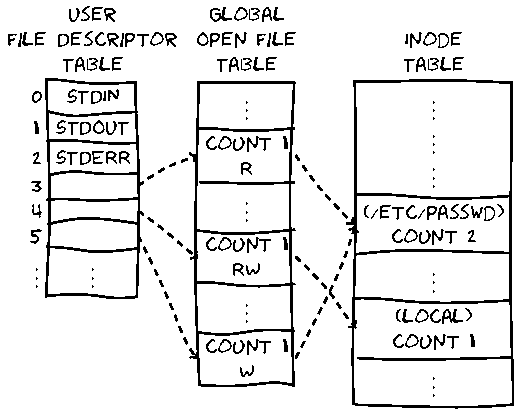
\includegraphics[width=.6\textwidth]{file-tables2} }%
    \mode<article>{ 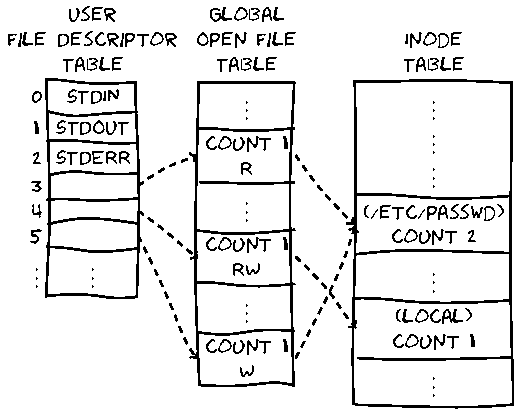
\includegraphics[width=.4\textwidth]{file-tables2} }
  \end{center}
\end{frame}

\begin{frame}
  \begin{iblock}{One more process B:}\ttfamily
    \begin{itemize}
    \item[] fd1 = open("/etc/passwd", O\_RDONLY);
    \item[] fd2 = open("private", O\_RDONLY);
    \end{itemize}
  \end{iblock}
  \begin{center}
    \mode<beamer>{ 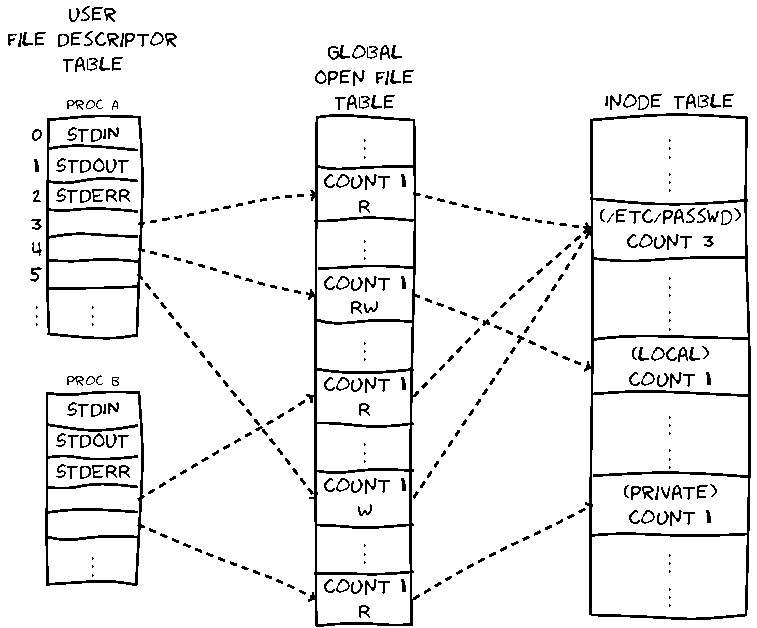
\includegraphics[width=.7\textwidth]{file-tables3} }%
    \mode<article>{ 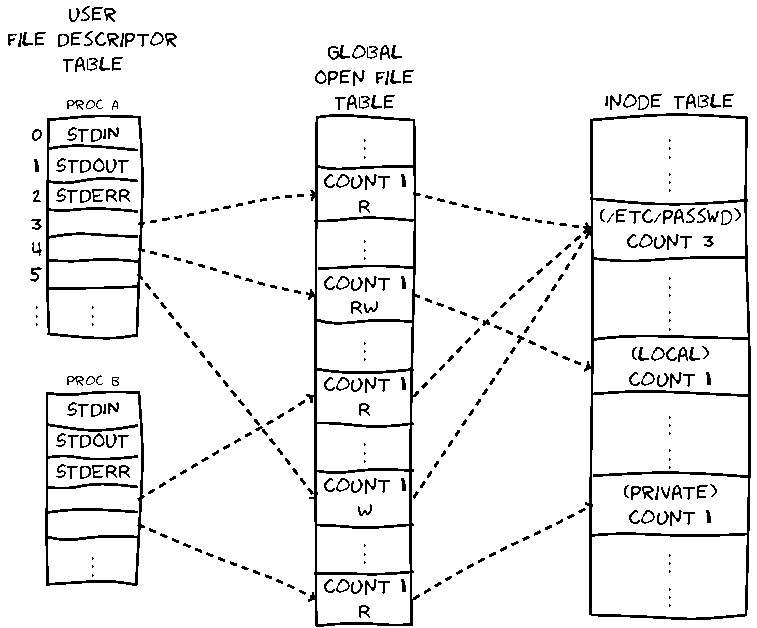
\includegraphics[width=.5\textwidth]{file-tables3} }
  \end{center}
\end{frame}

\section{Directories}

\begin{frame}{Implementing Directories}
  \begin{center}
    \mode<beamer>{ 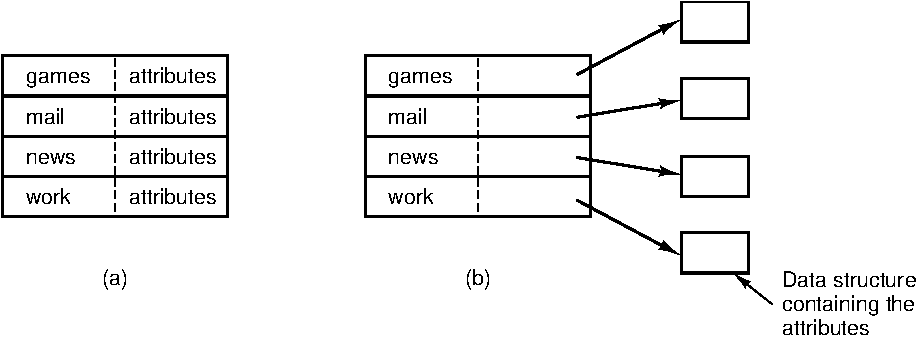
\includegraphics[width=\textwidth]{mos-figs-6-16} }%
    \mode<article>{ 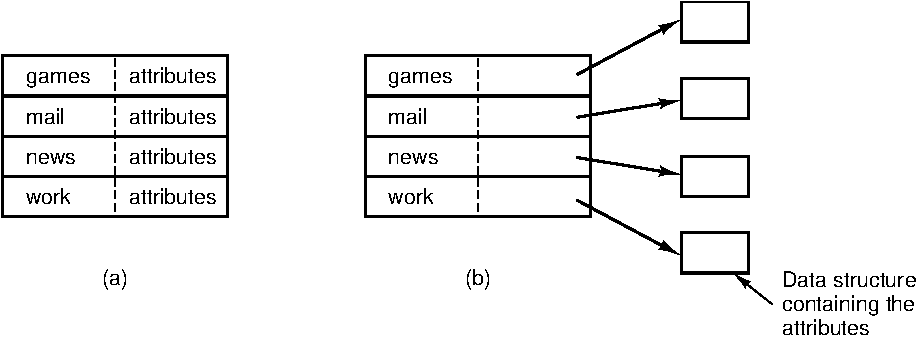
\includegraphics[width=.5\textwidth]{mos-figs-6-16} }
  \end{center}
  \begin{itemize}
  \item[(a)] A simple directory (Windows)
    \begin{itemize}
    \item fixed size entries
    \item disk addresses and attributes in directory entry
    \end{itemize}
  \item[(b)] Directory in which each entry just refers to an i-node (UNIX)
  \end{itemize}
\end{frame}

\begin{frame}%{Directory}
  \begin{iblock}{Directory entry in \texttt{glibc}}
    \mode<beamer>{ 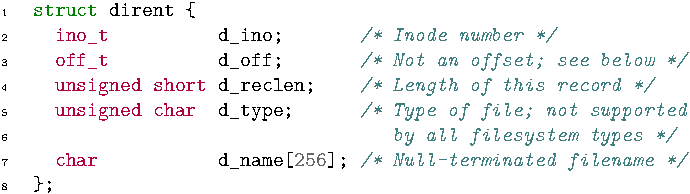
\includegraphics[width=\textwidth]{dirent-c} }%
    \mode<article>{\cfile{../src/dirent.c}}
  \end{iblock}
  \begin{itemize}
  \item[\$] \cmd{man readdir}
  \item[\$] \cmd{view /usr/include/x86\_64-linux-gnu/bits/dirent.h}
  \end{itemize}
\end{frame}

\begin{frame}{Ext2 Directories}
  \begin{center}
    \mode<beamer>{ \includegraphics[width=\textwidth]{ext2dir2} }%
    \mode<article>{ \includegraphics[width=.6\textwidth]{ext2dir2} }
  \end{center}
  \begin{minipage}{.39\textwidth}
    \begin{center}
      \mode<beamer>{ \includegraphics[width=\textwidth]{ext2dir} }%
      \mode<article>{ \includegraphics[width=.7\textwidth]{ext2dir} }
    \end{center}
  \end{minipage}\quad
  \begin{minipage}{.55\textwidth}
    \begin{itemize}
    \item Directories are special files
    \item ``\texttt{.}'' and ``\texttt{..}'' first
    \item Padding to $4\times{}$
    \item inode number is 0 --- deleted file
    \end{itemize}
  \end{minipage}
\end{frame}

\begin{frame}{\ttfamily ls}
  \mode<beamer>{%
    \begin{tikzpicture}[remember picture, overlay]%
      \node [scale=.27,opacity=.5,anchor=east] at (current page.east)%
      {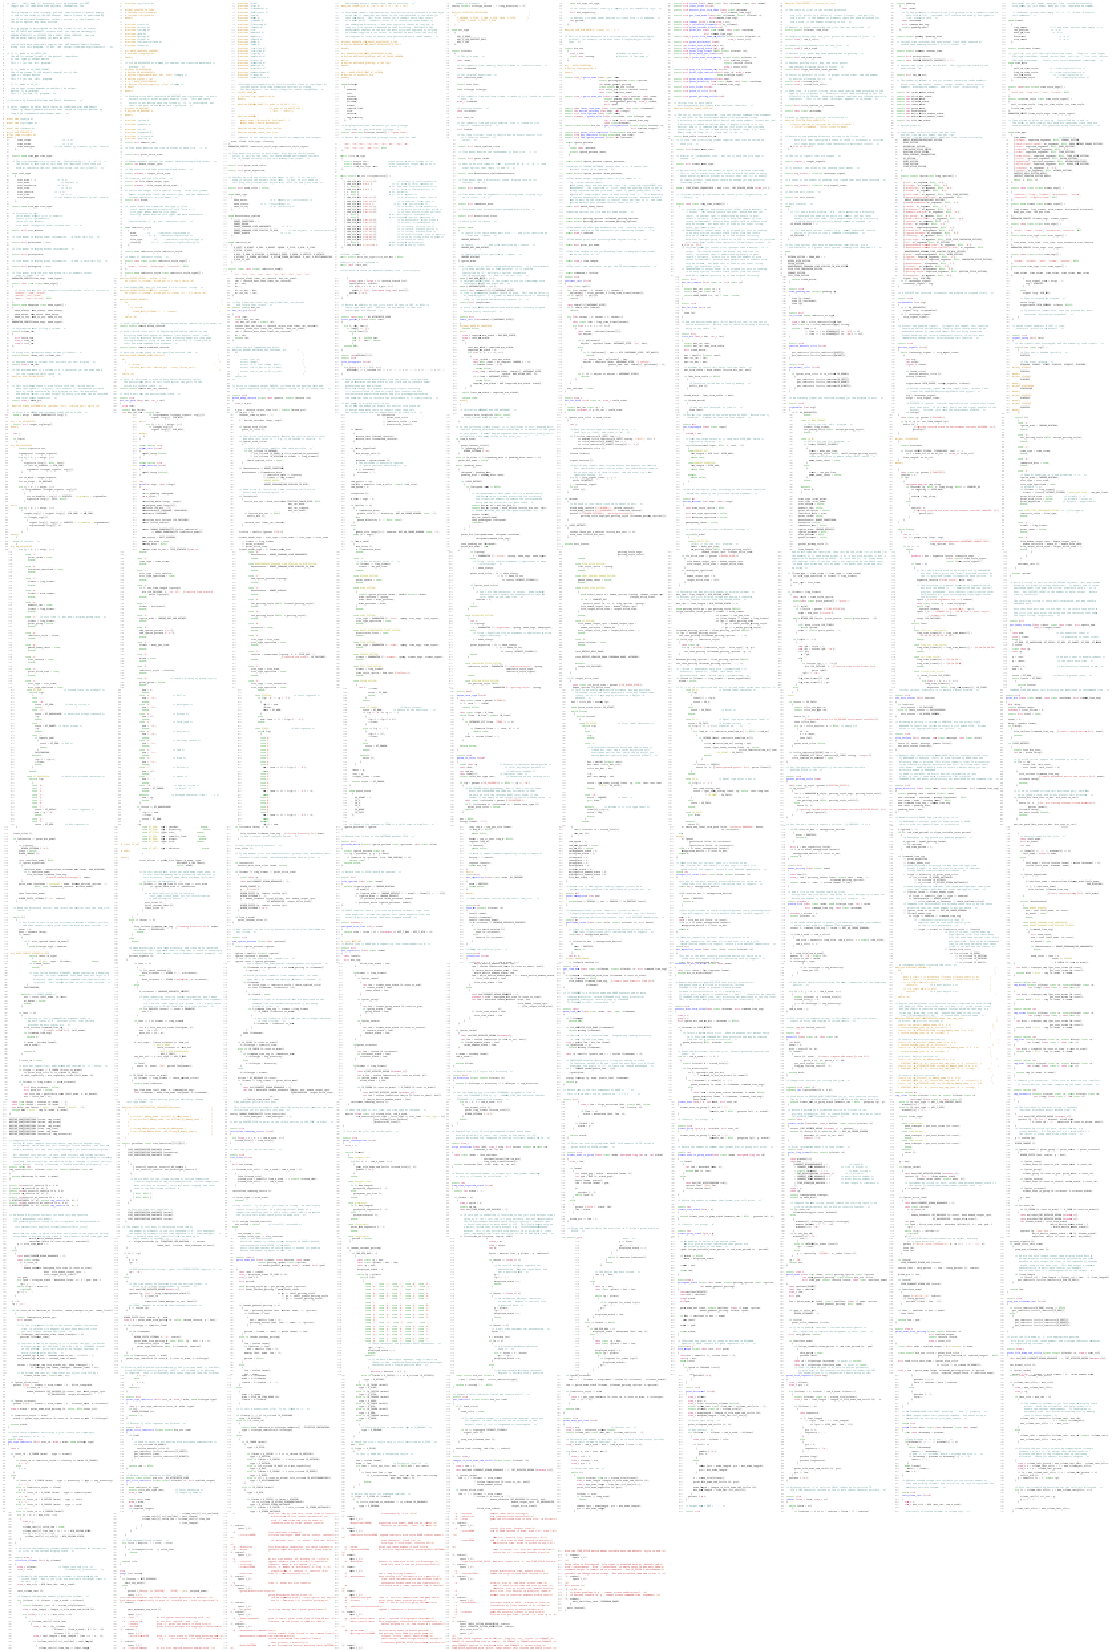
\includegraphics{ls-real}};
    \end{tikzpicture}}
  
  \begin{minipage}{.6\linewidth}
    \mode<beamer>{ \includegraphics[width=\textwidth]{ls-c} }%
    \mode<article>{\cfile{../src/ls.c}}
  \end{minipage}\quad
  \begin{minipage}{.35\linewidth}
    \begin{description}
    \item[The real \texttt{ls.c}?] 
    \end{description}
    \mode<beamer>{
    \begin{flushright}
      \begin{large}
        116 A4 pages\\
        5308 lines\\[1em]
        Do one thing, and do it really well.\\[2em]
      \end{large}
    \end{flushright}
    {\small \CMD{apt source coreutils}}}
  \mode<article>{
    \begin{itemize}
    \item 116 A4 pages
    \item 5308 lines
    \end{itemize}
    Do one thing, and do it really well.
    \begin{itemize}
    \item[\$] \cmd{apt source coreutils}
    \end{itemize}}
  \end{minipage}  
\end{frame}

\begin{frame}{\ttfamily mkdir(), chdir(), rmdir(), getcwd()}
  \begin{center}
    \mode<beamer>{ 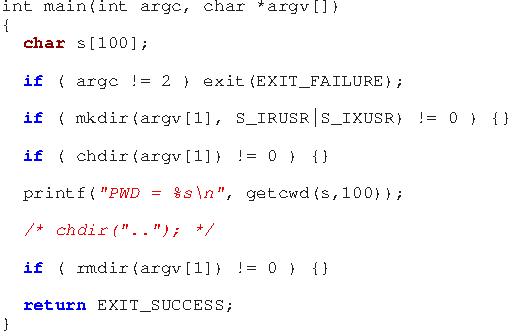
\includegraphics[width=.9\textwidth]{mkdir-c} }%
    \mode<article>{\cfile{../src/mkdir.c}}
  \end{center}
\end{frame}

\begin{frame}{Hard Links}
  \begin{iblock}{Hard links {\pright} the same inode}
    \begin{center}
      \mode<beamer>{ 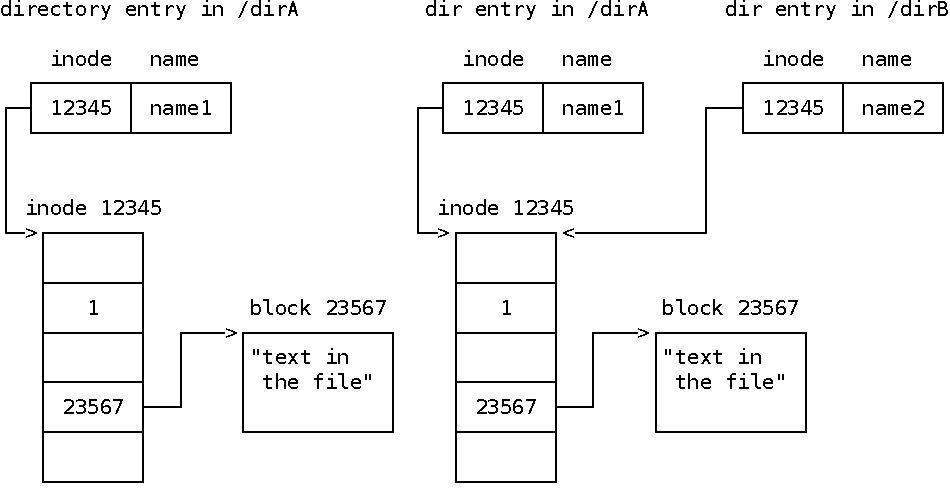
\includegraphics[width=\textwidth]{hard-link} }%
      \mode<article>{ 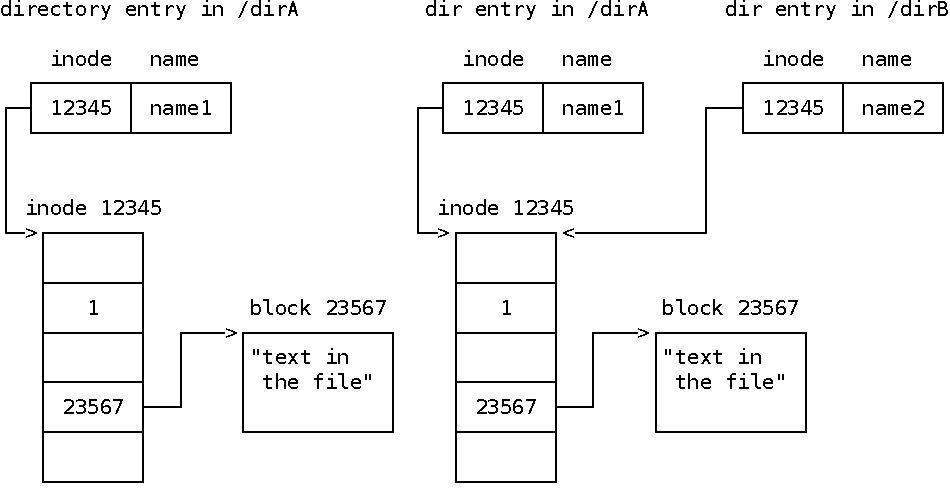
\includegraphics[width=.5\textwidth]{hard-link} }
    \end{center}
  \end{iblock}
\end{frame}

\begin{frame}
  \begin{iblock}{Drawback}
    \begin{center}
      \mode<beamer>{ 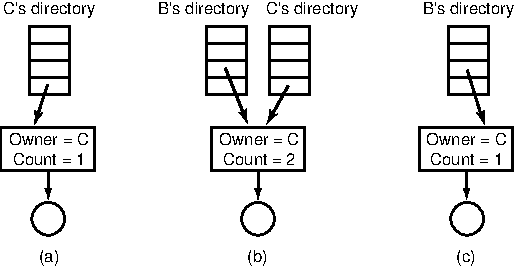
\includegraphics[width=\textwidth]{hardlink-drawback} }%
      \mode<article>{ 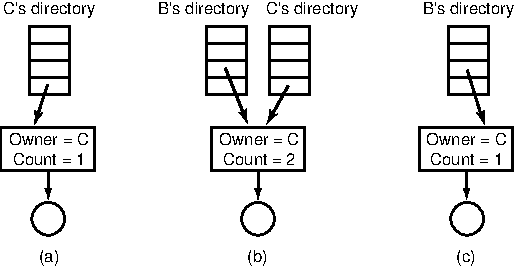
\includegraphics[width=.4\textwidth]{hardlink-drawback} }
    \end{center}
  \end{iblock}
\end{frame}

\begin{frame}{Symbolic Links}
  \begin{iblock}{A symbolic link has its own inode {\pright} a directory entry}
    \begin{center}
      \mode<beamer>{ \includegraphics[width=.9\textwidth]{soft-link} }%
      \mode<article>{ \includegraphics[width=.5\textwidth]{soft-link} }
    \end{center}
  \end{iblock}
  \begin{description}
  \item[Fast symbolic link:] Short path name ($< 60\,chars$) needs no data block. Can be
    stored in the 15 pointer fields
  \end{description}
\end{frame}

\begin{frame}{\ttfamily link(), unlink(), symlink()}
  \begin{center}
    \mode<beamer>{ 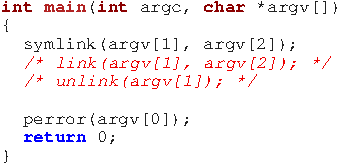
\includegraphics[width=.7\textwidth]{link-c} }%
    \mode<article>{\cfile{../src/link.c}}
  \end{center}
\end{frame}


\mode<all>
%%% Local Variables:
%%% mode: latex
%%% TeX-master: "lap-b"
%%% End:
